\documentclass{article}

\usepackage[utf8]{inputenc}
\usepackage{graphicx}
\usepackage{geometry}
\usepackage{xcolor}
\usepackage{titlesec}
\usepackage{fancyhdr}
\usepackage{tocloft}
\usepackage{float}

\geometry{margin=2.5cm}


\definecolor{myblue}{HTML}{2C56C9}
\definecolor{myline}{HTML}{253555}

\titleformat{\section}
{\color{myblue}\normalfont\Large\bfseries}
{\thesection}{1em}{}

\fancypagestyle{normal}{
    \fancyhf{}
    \fancyhead[L]{\textcolor{myblue}{Corsi di Studi in Informatica}}
    \fancyhead[R]{\textcolor{myblue}{00BD58}}
    \fancyfoot[L]{\textcolor{myblue}{UninaFoodLab}}
    \fancyfoot[C]{\thepage}
    \fancyfoot[R]{\textcolor{myblue}{2025/2026}}
    \renewcommand{\headrulewidth}{0.4pt}
    \renewcommand{\footrulewidth}{0.4pt}
    \renewcommand{\headrule}{\color{myline}\hrule height 0.4pt \vspace{3pt}}
    \renewcommand{\footrule}{\color{myline}\hrule height 0.4pt \vspace{3pt}}
}

\fancypagestyle{firstpage}{
    \fancyhf{}
    \fancyfoot[L]{\textcolor{myblue}{UninaFoodLab}}
    \fancyfoot[C]{\thepage}
    \fancyfoot[R]{\textcolor{myblue}{2025/2026}}
    \renewcommand{\headrulewidth}{0pt}
    \renewcommand{\footrulewidth}{0.4pt}
    \renewcommand{\footrule}{\color{myline}\hrule height 0.4pt \vspace{3pt}}
}



\renewcommand{\contentsname}{Indice}
\renewcommand{\cftsecfont}{\color{myblue}\bfseries}

\begin{document}



\thispagestyle{firstpage}


\begin{center}
    
\includegraphics[width=0.3\textwidth]{latex/immagini/uni_logo.png} 
    \vspace{0.5cm}

    {\large \textbf{Corso di Laurea in Informatica - Università degli Studi di Napoli Federico II}}\\
    {\large \textbf{A.A. 2025/2026}}\\[1cm]
    \vspace{1cm}

    {\Huge \color{myblue} \textbf{UninaFoodLab}}\\[2cm]

    \begin{flushleft}
    \centering
    {\large
    \textbf{Calone Francesco N86005555}\\
    \vspace{0.2cm}
    \textbf{D'Angelo Mario N86005477}\\
    }
    
    \vspace{0.2cm}
    {\small Codice gruppo: \textbf{OOBD39}}\\
    \vspace{0.8cm} 

    {\small Insegnamento di Programmazione Object-Oriented}
    \end{flushleft}
\end{center}


\newpage

\pagestyle{normal}

\tableofcontents
\thispagestyle{normal}

\section{Introduzione}

Il progetto UninaFoodLab nasce con l'obiettivo di offrire una soluzione software moderna e intuitiva per la gestione di corsi culinari. La piattaforma è stata sviluppata seguendo le best practice adottando tecnologie consolidate come JavaFX per la realizzazione dell'interfaccia grafica e Maven per la gestione delle dipendenze e dei processi di build.
Il progetto è stato concepito per essere facilmente estendibile e manutenibile, grazie a una chiara separazione dei livelli logici.
La documentazione che segue illustra le scelte progettuali, le tecnologie utilizzate e le principali funzionalità implementate, con l'intento di fornire una panoramica completa e professionale del sistema sviluppato.
\subsection{Obiettivi del Progetto}
Il progetto UninaFoodLab si propone di:
\begin{itemize}
    \item Fornire una piattaforma intuitiva per la gestione di corsi culinari
    \item Semplificare la registrazione e la gestione degli utenti e per gli chef
    \item Facilitare la creazione e la gestione dei corsi, inclusa la pianificazione delle lezioni e la gestione delle ricette
    \item Semplificare la gestione delle prenotazioni e dei pagamenti per i corsi
\end{itemize}

\section{progettazione concettuale}
\subsection{Introduzione}
Il modello concettuale rappresenta la struttura logica del database, definendo le entità, gli attributi e le relazioni tra di esse. In questa fase, si è proceduto a identificare le principali entità del sistema e a stabilire le relazioni che le collegano, garantendo così una visione chiara e coerente delle informazioni da gestire.
\subsection{UML non ristrutturato}
\begin{figure}[H]
    \noindent\makebox[\linewidth]{%
        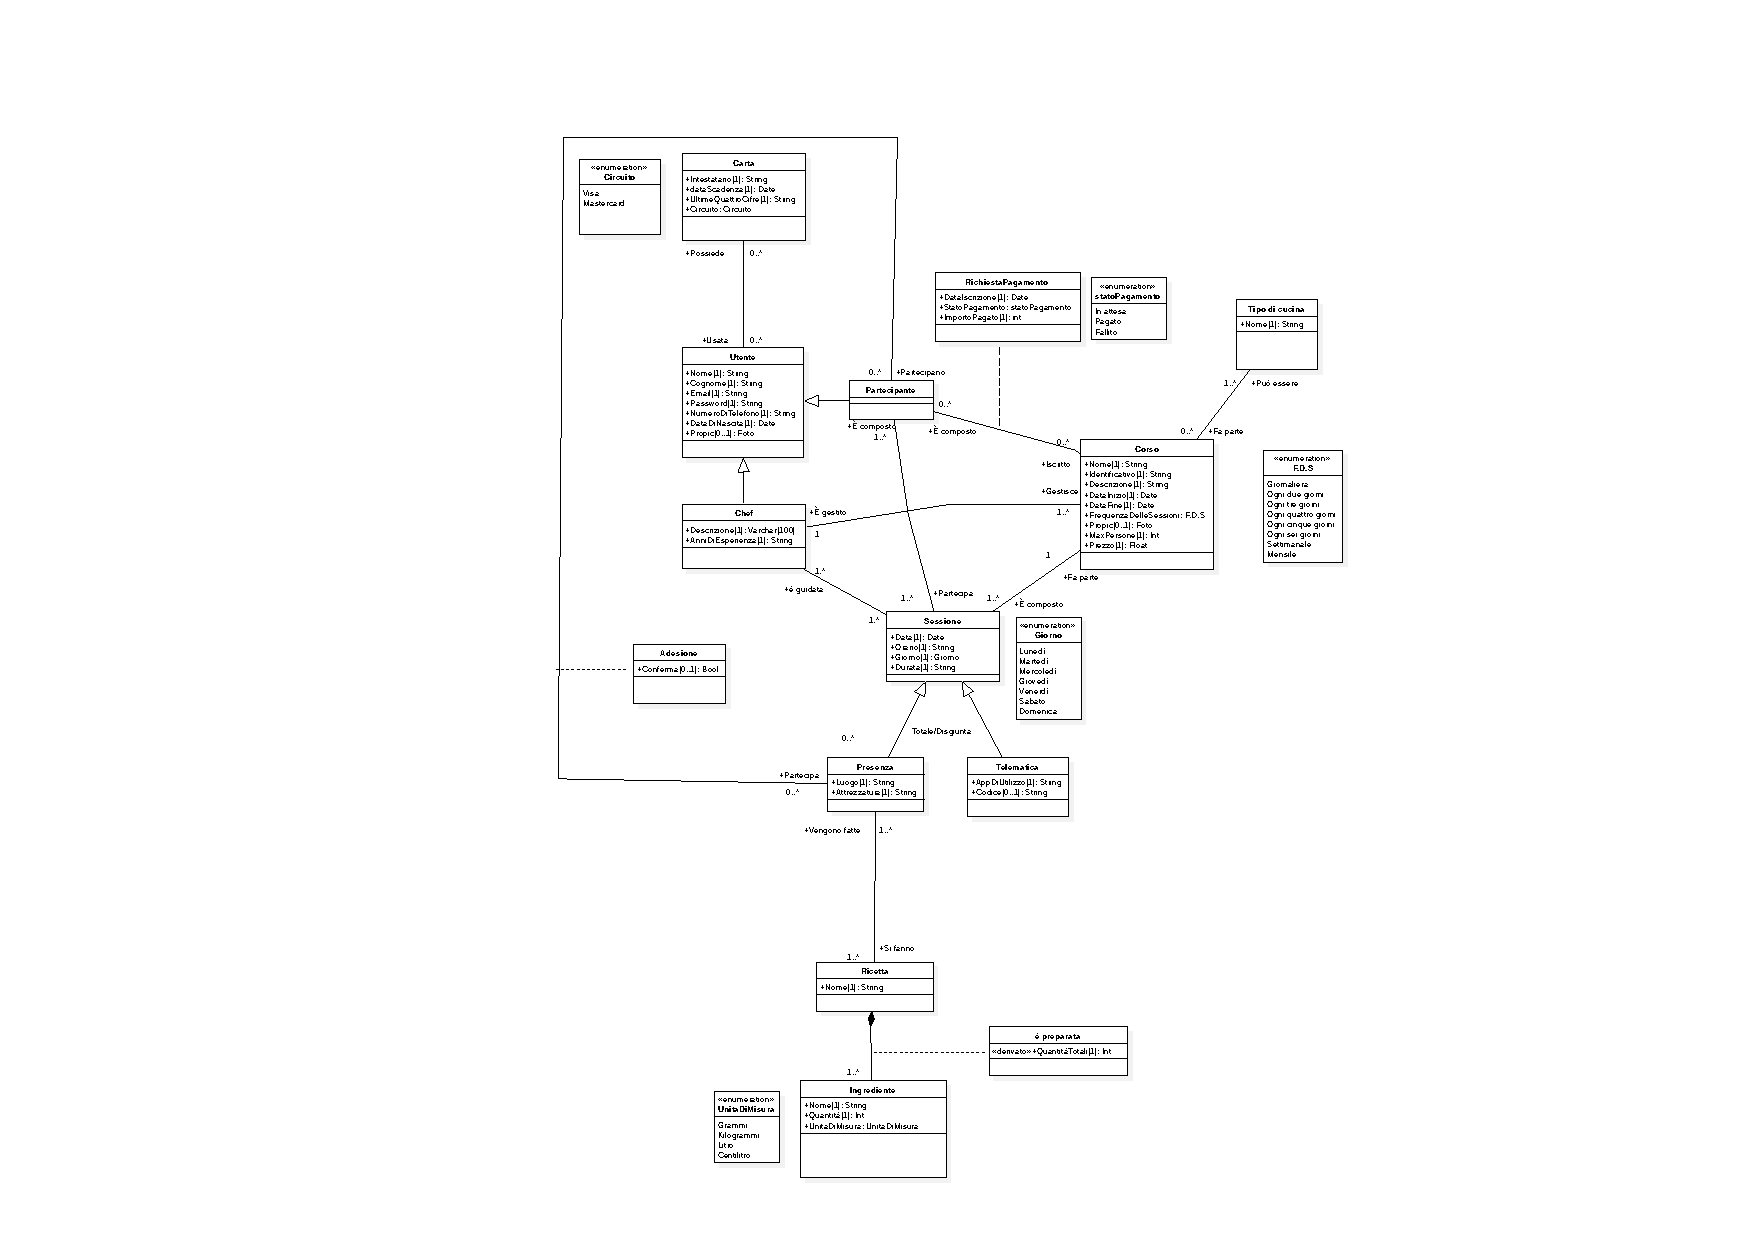
\includegraphics[height=0.9\textheight,width=2\textwidth]{latex/immagini/uml_non_ristrutturato.pdf}
    }
    \caption{Diagramma UML del sistema}
\end{figure}
\subsubsection{Entità principali}
Le entità principali identificate nel sistema sono:
\begin{itemize}
    \item \textbf{Utente}: L’utente rappresenta il soggetto fruitore del sistema, che può iscriversi ai corsi e partecipare alle sessioni. I principali attributi includono nome, cognome, email, password, telefono, data di nascita e una foto di profilo. Ogni utente può essere associato a una o più carte di pagamento e può diventare partecipante a diversi corsi.
    \item \textbf{Chef}: Lo chef è un utente con il ruolo specifico di organizzare corsi. Ogni chef dispone di una descrizione e di un numero di anni di esperienza. Un chef può gestire più corsi, ma ogni corso è gestito da un solo chef.
    \item \textbf{Corso}: Il corso è l'entità centrale del sistema e rappresenta una proposta didattica su un tema gastronomico specifico. Contiene attributi quali nome, descrizione, identificativo, data di inizio/fine, frequenza delle sessioni, prezzo, immagine di copertina e tipo di cucina (modellato come enumerazione). Ogni corso è composto da più sessioni e prevede una relazione molti-a-molti con i partecipanti.
    \item \textbf{Sessione}: Ogni corso è articolato in una o più sessioni, ciascuna delle quali ha una data, un orario, un insieme di giorni della settimana in cui si svolge, e una durata. Le sessioni sono specializzate in due sottotipi mutuamente esclusivi:
    \begin{itemize}
        \item \textbf{Presenza}: Con attributi come luogo e attrezzature richieste.
        \item \textbf{Telematica}: Con attributi relativi all'app utilizzata e al codice di accesso.
    \end{itemize}
    \item \textbf{Partecipante e Adesione}: La partecipazione ai corsi è modellata tramite l’entità Partecipante, che collega utenti e corsi. La partecipazione a sessioni pratiche richiede un’adesione esplicita, rappresentata dall'entità Adesione, che contiene un attributo booleano di conferma.
    \item \textbf{Ricetta e Ingredientemento}: Ogni sessione pratica può includere la preparazione di una o più ricette. Ogni ricetta è composta da uno o più ingredienti, ciascuno dei quali ha un nome, una quantità e un'unità di misura (enumerata). La relazione tra Ricetta e Ingrediente è associativa e include l'attributo QuantitàTotale, utile per calcolare la quantità necessaria in base alle adesioni.
    \item \textbf{Carta e RichiestaPagamento}: Gli utenti possono associare al proprio profilo una o più carte di pagamento, appartenenti a un circuito specificato tramite enumerazione (Visa, Mastercard). Le richieste di pagamento sono entità separate, con data, stato (in attesa, pagato, fallito) e importo.
\end{itemize}
\subsubsection{Gerarchie e generalizzazioni}
Nel modello concettuale, sono state identificate le seguenti gerarchie e generalizzazioni:
\begin{itemize}
    \item \textbf{Sessione}: Le sessioni sono suddivise in due sottotipi: \textit{Presenza} e \textit{Telematica}. Questa specializzazione consente di gestire le specificità di ciascun tipo di sessione, come il luogo e le attrezzature per le sessioni in presenza, e l'app utilizzata e il codice di accesso per quelle telematiche.
    \item \textbf{Utente}: L'entità Utente può essere specializzata in due sottotipi: \textit{Partecipante} e \textit{Chef}. Questa distinzione permette di gestire le diverse funzionalità e attributi associati a ciascun ruolo nel sistema.
\end{itemize}
Entrambe le specializzazioni sono totali e disgiunte, di conseguenza ogni istanza di Sessione sia esclusivamente di uno dei due tipi e che ogni Utente sia o un Partecipante o uno Chef, ma non entrambi contemporaneamente.
\subsubsection{Relazioni tra le entità}
Le relazioni tra le entità sono state definite come segue:
\begin{itemize}
    \item \textbf{Utente - Partecipante}: Un utente può essere un partecipante a più corsi, e ogni corso può avere più partecipanti. Questa relazione è molti-a-molti.
    \item \textbf{Chef - Corso}: Ogni chef può gestire più corsi, ma ogni corso è associato a un solo chef. Questa relazione è uno-a-molti.
    \item \textbf{Corso - Sessione}: Un corso può avere più sessioni, ma ogni sessione appartiene a un solo corso. Questa relazione è uno-a-molti.
    \item \textbf{Sessione - Partecipante}: Ogni partecipante può aderire a più sessioni pratiche, e ogni sessione può avere più partecipanti. Questa relazione è molti-a-molti, mediata dall'entità Adesione.
    \item \textbf{Corso - Ricetta}: Ogni corso può includere più ricette, e ogni ricetta può essere associata a più corsi. Questa relazione è molti-a-molti.
    \item \textbf{Ricetta - Ingrediente}: Ogni ricetta può includere più ingredienti, e ogni ingrediente può essere utilizzato in più ricette. Questa relazione è molti-a-molti, mediata dall'attributo QuantitàTotale.
    \item \textbf{Utente - Carta}: Un utente può avere più carte di pagamento associate al proprio profilo. Questa relazione è uno-a-molti.
    \item \textbf{Ricetta - Ingrediente}: Ogni ricetta può essere associata a più ingredienti, e ogni ingrediente può essere utilizzato in più ricette. Questa relazione è una composizione, mediata dall'attributo QuantitàTotale.
\end{itemize}
\subsubsection{Motivazione delle scelte progettuali}
Le scelte progettuali sono state guidate dalla necessità di garantire una rappresentazione chiara e coerente delle informazioni, facilitando la gestione dei corsi, delle sessioni e delle partecipazioni. La specializzazione delle sessioni in Presenza e Telematica consente di gestire le specificità di ciascun tipo di sessione, mentre la distinzione tra Partecipante e Chef permette di differenziare i ruoli degli utenti nel sistema. Inoltre, l'uso di relazioni molti-a-molti per gestire le adesioni alle sessioni pratiche e le associazioni tra ricette e ingredienti garantisce flessibilità e scalabilità nel modello.



\section{Architettura del Progetto}

L'architettura del progetto UninaFoodLab è stata progettata per garantire una chiara separazione dei compiti e una facile manutenibilità. La struttura delle directory riflette i principali livelli logici dell'applicazione, secondo il pattern MVC e le best practice di progettazione.

Le principali suddivisioni sono:
\begin{itemize}
    \item \textbf{Boundary}: contiene le classi responsabili dell'interfaccia grafica e dell'interazione con l'utente, realizzate tramite JavaFX e FXML.
    \item \textbf{Controller}: gestisce la logica applicativa e il flusso degli eventi tra la GUI e i dati.
    \item \textbf{Entity}: suddivisa ulteriormente in \textit{DAO} (Data Access Object) e \textit{DTO} (Data Transfer Object). I DAO si occupano della persistenza e dell'accesso ai dati, mentre i DTO rappresentano le strutture dati scambiate tra i vari livelli.
    \item \textbf{JDBC}: contiene le classi e le utility per la connessione e la gestione del database PostgreSQL.
    \item \textbf{Utils}: raccoglie le classi di supporto e gli strumenti riutilizzabili all'interno del progetto.
\end{itemize}
Questa organizzazione favorisce la modularità e la scalabilità del sistema, permettendo di isolare le responsabilità e facilitare l'estensione futura. Ogni componente interagisce con gli altri tramite interfacce ben definite, riducendo le dipendenze e migliorando la qualità del codice.

La scelta di suddividere le entity in DAO e DTO consente di gestire in modo efficiente sia la persistenza che il trasferimento dei dati, mentre la presenza di una directory dedicata alle utility semplifica la gestione delle funzionalità trasversali.

\subsection{Struttura delle Directory}
La struttura delle directory del progetto è organizzata come segue:
\begin{itemize}
    \item \textbf{src/main/java}: contiene il codice sorgente dell'applicazione.
    \item \textbf{src/main/resources}: contiene le risorse dell'applicazione, come file FXML e immagini.
    \item \textbf{src/test/java}: contiene i test automatizzati.
\end{itemize}


\section{Definizioni SQL}

\subsection{Introduzione}

In questo capitolo viene presentata l'implementazione pratica del database UninaFoodLab attraverso la definizione completa del codice SQL sviluppato in PostgreSQL. La sezione fornisce una panoramica dettagliata di tutti gli elementi che compongono il database, dalla creazione delle tabelle all'implementazione delle funzioni.


\subsection{Definizione degli enumerati}

Gli enumerati sono tipi di dato definiti dall’utente che permettono di vincolare il valore di un attributo a un insieme finito di possibilità predefinite. Nel database UninaFoodLab vengono utilizzati per rappresentare domini chiusi come circuiti di carte, stati di pagamento, frequenza delle sessioni, giorni della settimana e unità di misura degli ingredienti. Questo garantisce coerenza e integrità dei dati, semplificando la gestione delle regole applicative.

\noindent\rule{\textwidth}{0.4pt}
\begin{lstlisting}[language=SQL, style=sqlstyle, literate={à}{{\`a}}1 {è}{{\`e}}1 {é}{{\'e}}1 {ì}{{\`i}}1 {ò}{{\`o}}1 {ù}{{\`u}}1]
CREATE TYPE Circuito AS ENUM ('Visa', 'Mastercard');

CREATE TYPE StatoPagamento AS ENUM ('In attesa', 'Pagato', 'Fallito');

CREATE TYPE FDS AS ENUM (
  'Giornaliera',
  'Ogni due giorni',
  'Ogni tre giorni',
  'Ogni quattro giorni',
  'Ogni cinque giorni',
  'Ogni sei giorni',
  'Settimanale',
  'Mensile'
);

CREATE TYPE Giorno AS ENUM (
  'Lunedì',
  'Martedì',
  'Mercoledì',
  'Giovedì',
  'Venerdì',
  'Sabato',
  'Domenica'
);

CREATE TYPE UnitaDiMisura AS ENUM ('Grammi', 'Kilogrammi', 'Litro', 'Centilitro');
\end{lstlisting}
\noindent\rule{\textwidth}{0.4pt}

\subsection{Definizione delle Tabelle}


\subsubsection{Tabella Partecipante}

La tabella \texttt{Partecipante} rappresenta gli utenti che si iscrivono e partecipano ai corsi di cucina. Ogni partecipante ha un identificativo univoco generato automaticamente e deve fornire informazioni personali essenziali per la registrazione.

\noindent\rule{\textwidth}{0.4pt}
\begin{lstlisting}[language=SQL, style=sqlstyle]
CREATE TABLE Partecipante (
    IdPartecipante INT GENERATED ALWAYS AS IDENTITY PRIMARY KEY,
    Nome VARCHAR(50) NOT NULL,
    Cognome VARCHAR(50) NOT NULL,
    Email VARCHAR(100) UNIQUE NOT NULL,
    Password VARCHAR(100) NOT NULL,
    DataDiNascita DATE NOT NULL,
    Propic TEXT
);
\end{lstlisting}
\noindent\rule{\textwidth}{0.4pt}

\textbf{Scelte progettuali:}
\begin{itemize}
    \item \textbf{IdPartecipante}: Chiave primaria auto-incrementale utilizzando \texttt{GENERATED ALWAYS AS IDENTITY} per garantire unicità automatica
    \item \textbf{Email}: Constraint \texttt{UNIQUE} per evitare registrazioni duplicate
    \item \textbf{Password}: Campo di lunghezza fissa per supportare hash di password sicure
    \item \textbf{Propic}: Campo \texttt{TEXT} per supportare URL di immagini o dati base64
\end{itemize}

\subsubsection{Tabella Carta}

La tabella \texttt{Carta} memorizza le carte di pagamento associate agli utenti. Ogni carta ha un identificativo univoco, intestatario, data di scadenza, ultime quattro cifre e circuito di appartenenza.

\noindent\rule{\textwidth}{0.4pt}
\begin{lstlisting}[language=SQL, style=sqlstyle]
CREATE TABLE Carta (
    IdCarta INT GENERATED ALWAYS AS IDENTITY PRIMARY KEY,
    Intestatario VARCHAR(100) NOT NULL,
    DataScadenza DATE NOT NULL,
    UltimeQuattroCifre CHAR(4) NOT NULL,
    Circuito VARCHAR(50) NOT NULL
);
\end{lstlisting}
\noindent\rule{\textwidth}{0.4pt}

\textbf{Scelte progettuali:}
\begin{itemize}
    \item \textbf{IdCarta}: Chiave primaria auto-incrementale
    \item \textbf{Intestatario, DataScadenza, UltimeQuattroCifre, Circuito}: Attributi essenziali per identificare una carta
    \item \textbf{Circuito}: Vincolato tramite tipo enumerato per coerenza
\end{itemize}

\subsubsection{Tabella Possiede}

La tabella \texttt{Possiede} rappresenta la relazione molti-a-molti tra partecipanti e carte, indicando quali carte sono possedute da ciascun partecipante.

\noindent\rule{\textwidth}{0.4pt}
\begin{lstlisting}[language=SQL, style=sqlstyle]
CREATE TABLE Possiede (
    IdPartecipante INT,
    IdCarta INT,
    PRIMARY KEY (IdPartecipante, IdCarta),
    FOREIGN KEY (IdPartecipante) REFERENCES Partecipante(IdPartecipante),
    FOREIGN KEY (IdCarta) REFERENCES Carta(IdCarta) on delete cascade 
);
\end{lstlisting}
\noindent\rule{\textwidth}{0.4pt}

\textbf{Scelte progettuali:}
\begin{itemize}
    \item \textbf{Chiave primaria composta}: (IdPartecipante, IdCarta) per garantire unicità della relazione
    \item \textbf{Vincoli di integrità}: Foreign key verso \texttt{Partecipante} e \texttt{Carta}
    \item \textbf{Cascata}: Eliminazione a cascata delle carte
\end{itemize}

\subsubsection{Tabella Corso}

La tabella \texttt{Corso} rappresenta i corsi di cucina offerti, con informazioni su nome, descrizione, periodo, frequenza, prezzo, chef responsabile e limiti di partecipazione.

\noindent\rule{\textwidth}{0.4pt}
\begin{lstlisting}[language=SQL, style=sqlstyle]
CREATE TABLE Corso (
    IdCorso INT GENERATED ALWAYS AS IDENTITY PRIMARY KEY,
    Nome VARCHAR(100) NOT NULL,
    Descrizione VARCHAR(60) NOT NULL,
    DataInizio DATE NOT NULL,
    DataFine DATE NOT NULL,
    FrequenzaDelleSessioni VARCHAR(100) NOT NULL,
    Propic TEXT,
    MaxPersone INT CHECK (MaxPersone > 0),
    Prezzo DECIMAL(10, 2) CHECK (Prezzo >= 0),
    IdChef INT NOT NULL,
    FOREIGN KEY (IdChef) REFERENCES Chef(IdChef)
);
\end{lstlisting}
\noindent\rule{\textwidth}{0.4pt}

\textbf{Scelte progettuali:}
\begin{itemize}
    \item \textbf{IdCorso}: Chiave primaria auto-incrementale
    \item \textbf{MaxPersone, Prezzo}: Vincoli di validità sui valori
    \item \textbf{IdChef}: Foreign key verso chef responsabile
    \item \textbf{FrequenzaDelleSessioni}: Vincolata tramite tipo enumerato
\end{itemize}

\subsubsection{Tabella RichiestaPagamento}

La tabella \texttt{RichiestaPagamento} registra le richieste di pagamento per i corsi, associando ogni richiesta a un partecipante e a un corso specifico, con informazioni su importo, stato e data.

\noindent\rule{\textwidth}{0.4pt}
\begin{lstlisting}[language=SQL, style=sqlstyle]
CREATE TABLE RichiestaPagamento (
    DataRichiesta TIMESTAMP NOT NULL,
    StatoPagamento VARCHAR(50) NOT NULL,
    ImportoPagato DECIMAL(10, 2) CHECK (ImportoPagato >= 0),
    IdCorso INT,
    IdPartecipante INT,
    PRIMARY KEY (DataRichiesta, IdCorso, IdPartecipante),
    FOREIGN KEY (IdCorso) REFERENCES Corso(IdCorso),
    FOREIGN KEY (IdPartecipante) REFERENCES Partecipante(IdPartecipante)
);
\end{lstlisting}
\noindent\rule{\textwidth}{0.4pt}

\textbf{Scelte progettuali:}
\begin{itemize}
    \item \textbf{Chiave primaria composta}: (DataRichiesta, IdCorso, IdPartecipante)
    \item \textbf{ImportoPagato}: Vincolo di non negatività
    \item \textbf{StatoPagamento}: Vincolato tramite tipo enumerato
    \item \textbf{Foreign key}: Collegamento a corso e partecipante
\end{itemize}

\subsubsection{Tabella TipoDiCucina}

La tabella \texttt{TipoDiCucina} elenca le tipologie di cucina disponibili, ciascuna con un identificativo univoco e un nome.

\noindent\rule{\textwidth}{0.4pt}
\begin{lstlisting}[language=SQL, style=sqlstyle]
CREATE TABLE TipoDiCucina (
    IDTipoCucina INT GENERATED ALWAYS AS IDENTITY PRIMARY KEY,
    Nome VARCHAR(50) NOT NULL UNIQUE
);
\end{lstlisting}
\noindent\rule{\textwidth}{0.4pt}

\textbf{Scelte progettuali:}
\begin{itemize}
    \item \textbf{IDTipoCucina}: Chiave primaria auto-incrementale
    \item \textbf{Nome}: Unicità per evitare duplicati
\end{itemize}

\subsubsection{Tabella TipoDiCucina\_Corso}

La tabella \texttt{TipoDiCucina\_Corso} rappresenta l'associazione tra corsi e tipologie di cucina, permettendo di collegare più tipi di cucina a ciascun corso (fino a un massimo di due).

\noindent\rule{\textwidth}{0.4pt}
\begin{lstlisting}[language=SQL, style=sqlstyle]
CREATE TABLE TipoDiCucina_Corso (
    IDTipoCucina INT,
    IDCorso INT,
    PRIMARY KEY (IDTipoCucina, IDCorso),
    FOREIGN KEY (IDTipoCucina) REFERENCES TipoDiCucina(IDTipoCucina),
    FOREIGN KEY (IDCorso) REFERENCES Corso(IdCorso)
);
\end{lstlisting}
\noindent\rule{\textwidth}{0.4pt}

\textbf{Scelte progettuali:}
\begin{itemize}
    \item \textbf{Chiave primaria composta}: (IDTipoCucina, IDCorso)
    \item \textbf{Foreign key}: Collegamento a tipo di cucina e corso
    \item \textbf{Vincolo applicativo}: Massimo due tipi di cucina per corso (gestito da trigger)
\end{itemize}

\subsubsection{Tabella Chef}

La tabella \texttt{Chef} contiene le informazioni sugli chef che tengono i corsi. Oltre ai dati anagrafici, include una descrizione e gli anni di esperienza.

\noindent\rule{\textwidth}{0.4pt}
\begin{lstlisting}[language=SQL, style=sqlstyle]
CREATE TABLE Chef (
    IdChef INT GENERATED ALWAYS AS IDENTITY PRIMARY KEY,
    Nome VARCHAR(50) NOT NULL,
    Cognome VARCHAR(50) NOT NULL,
    Email VARCHAR(100) UNIQUE NOT NULL,
    Password VARCHAR(100) NOT NULL,
    DataDiNascita DATE NOT NULL,
    Descrizione VARCHAR(60),
    Propic TEXT,
    AnniDiEsperienza INT CHECK (AnniDiEsperienza >= 0)
);
\end{lstlisting}
\noindent\rule{\textwidth}{0.4pt}

\textbf{Scelte progettuali:}
\begin{itemize}
    \item \textbf{IdChef}: Chiave primaria auto-incrementale
    \item \textbf{Email}: Unicità per evitare duplicati
    \item \textbf{AnniDiEsperienza}: Vincolo di non negatività
    \item \textbf{Propic}: Supporto per immagine profilo
\end{itemize}

\subsubsection{Tabella Sessione\_Presenza}

La tabella \texttt{Sessione\_Presenza} descrive le sessioni in presenza dei corsi, con dettagli su luogo, data, orario, durata e chef responsabile.

\noindent\rule{\textwidth}{0.4pt}
\begin{lstlisting}[language=SQL, style=sqlstyle]
CREATE TABLE Sessione_Presenza (
    IdSessionePresenza INT GENERATED ALWAYS AS IDENTITY PRIMARY KEY,
    Giorno VARCHAR(20) NOT NULL,
    Data DATE NOT NULL,
    Orario TIME NOT NULL,
    Durata INTERVAL NOT NULL,
    Citta VARCHAR(50) NOT NULL,
    Via VARCHAR(100) NOT NULL,
    Cap CHAR(5) NOT NULL,
    Descrizione VARCHAR(60) NOT NULL,
    IdCorso INT,
    IdChef INT,
    FOREIGN KEY (IdCorso) REFERENCES Corso(IdCorso),
    FOREIGN KEY (IdChef) REFERENCES Chef(IdChef)
);
\end{lstlisting}
\noindent\rule{\textwidth}{0.4pt}

\textbf{Scelte progettuali:}
\begin{itemize}
    \item \textbf{IdSessionePresenza}: Chiave primaria auto-incrementale
    \item \textbf{Attributi luogo}: Città, via, cap per identificare la sede
    \item \textbf{Foreign key}: Collegamento a corso e chef
\end{itemize}

\subsubsection{Tabella Adesione\_SessionePresenza}

La tabella \texttt{Adesione\_SessionePresenza} registra l'adesione dei partecipanti alle sessioni in presenza, con conferma di partecipazione.

\noindent\rule{\textwidth}{0.4pt}
\begin{lstlisting}[language=SQL, style=sqlstyle]
CREATE TABLE Adesione_SessionePresenza (
    Conferma BOOLEAN,
    IdSessionePresenza INT,
    IdPartecipante INT,
    PRIMARY KEY (IdSessionePresenza, IdPartecipante),
    FOREIGN KEY (IdSessionePresenza) REFERENCES Sessione_Presenza(IdSessionePresenza),
    FOREIGN KEY (IdPartecipante) REFERENCES Partecipante(IdPartecipante)
);
\end{lstlisting}
\noindent\rule{\textwidth}{0.4pt}

\textbf{Scelte progettuali:}
\begin{itemize}
    \item \textbf{Chiave primaria composta}: (IdSessionePresenza, IdPartecipante)
    \item \textbf{Conferma}: Indica la presenza effettiva
    \item \textbf{Foreign key}: Collegamento a sessione presenza e partecipante
\end{itemize}

\subsubsection{Tabella Sessione\_Telematica}

La tabella \texttt{Sessione\_Telematica} descrive le sessioni online dei corsi, con dettagli su applicazione, codice chiamata, data, orario, durata e chef responsabile.

\noindent\rule{\textwidth}{0.4pt}
\begin{lstlisting}[language=SQL, style=sqlstyle]
CREATE TABLE Sessione_Telematica (
    IdSessioneTelematica INT GENERATED ALWAYS AS IDENTITY PRIMARY KEY,
    Applicazione VARCHAR(100) NOT NULL,
    CodiceChiamata VARCHAR(100) NOT NULL,
    Data DATE NOT NULL,
    Orario TIME NOT NULL,
    Durata INTERVAL NOT NULL,
    Giorno VARCHAR(20) NOT NULL,
    Descrizione VARCHAR(60) NOT NULL,
    IdCorso INT,
    IdChef INT,
    FOREIGN KEY (IdCorso) REFERENCES Corso(IdCorso),
    FOREIGN KEY (IdChef) REFERENCES Chef(IdChef)
);
\end{lstlisting}
\noindent\rule{\textwidth}{0.4pt}

\textbf{Scelte progettuali:}
\begin{itemize}
    \item \textbf{IdSessioneTelematica}: Chiave primaria auto-incrementale
    \item \textbf{Applicazione, CodiceChiamata}: Dettagli per l'accesso online
    \item \textbf{Foreign key}: Collegamento a corso e chef
\end{itemize}

\subsubsection{Tabella Partecipante\_SessioneTelematica}

La tabella \texttt{Partecipante\_SessioneTelematica} rappresenta la partecipazione dei partecipanti alle sessioni telematiche, associando ogni partecipante a una specifica sessione online.

\noindent\rule{\textwidth}{0.4pt}
\begin{lstlisting}[language=SQL, style=sqlstyle]
CREATE TABLE Partecipante_SessioneTelematica (
    IdPartecipante INT,
    IdSessioneTelematica INT,
    PRIMARY KEY (IdPartecipante, IdSessioneTelematica),
    FOREIGN KEY (IdPartecipante) REFERENCES Partecipante(IdPartecipante),
    FOREIGN KEY (IdSessioneTelematica) REFERENCES Sessione_Telematica(IdSessioneTelematica)
);
\end{lstlisting}
\noindent\rule{\textwidth}{0.4pt}

\textbf{Scelte progettuali:}
\begin{itemize}
    \item \textbf{Chiave primaria composta}: (IdPartecipante, IdSessioneTelematica)
    \item \textbf{Foreign key}: Collegamento a partecipante e sessione telematica
\end{itemize}

\subsubsection{Tabella Ricetta}

La tabella \texttt{Ricetta} contiene le ricette che possono essere preparate durante le sessioni dei corsi.

\noindent\rule{\textwidth}{0.4pt}
\begin{lstlisting}[language=SQL, style=sqlstyle]
CREATE TABLE Ricetta (
    IdRicetta INT GENERATED ALWAYS AS IDENTITY PRIMARY KEY,
    Nome VARCHAR(100) NOT NULL
);
\end{lstlisting}
\noindent\rule{\textwidth}{0.4pt}

\textbf{Scelte progettuali:}
\begin{itemize}
    \item \textbf{IdRicetta}: Chiave primaria auto-incrementale
    \item \textbf{Nome}: Nome della ricetta, obbligatorio
\end{itemize}

\subsubsection{Tabella Sessione\_Presenza\_Ricetta}

La tabella \texttt{Sessione\_Presenza\_Ricetta} associa le ricette alle sessioni in presenza, indicando quali ricette vengono preparate in ciascuna sessione.

\noindent\rule{\textwidth}{0.4pt}
\begin{lstlisting}[language=SQL, style=sqlstyle]
CREATE TABLE Sessione_Presenza_Ricetta (
    IdRicetta INT,
    IdSessionePresenza INT,
    PRIMARY KEY (IdRicetta, IdSessionePresenza),
    FOREIGN KEY (IdRicetta) REFERENCES Ricetta(IdRicetta),
    FOREIGN KEY (IdSessionePresenza) REFERENCES Sessione_Presenza(IdSessionePresenza)
);
\end{lstlisting}
\noindent\rule{\textwidth}{0.4pt}

\textbf{Scelte progettuali:}
\begin{itemize}
    \item \textbf{Chiave primaria composta}: (IdRicetta, IdSessionePresenza)
    \item \textbf{Foreign key}: Collegamento a ricetta e sessione presenza
\end{itemize}

\subsubsection{Tabella Ingrediente}

La tabella \texttt{Ingrediente} elenca tutti gli ingredienti disponibili, con nome e unità di misura.

\noindent\rule{\textwidth}{0.4pt}
\begin{lstlisting}[language=SQL, style=sqlstyle]
CREATE TABLE Ingrediente (
    IdIngrediente INT GENERATED ALWAYS AS IDENTITY PRIMARY KEY,
    Nome VARCHAR(100) NOT NULL,
    UnitaDiMisura VARCHAR(50) NOT NULL
);
\end{lstlisting}
\noindent\rule{\textwidth}{0.4pt}

\textbf{Scelte progettuali:}
\begin{itemize}
    \item \textbf{IdIngrediente}: Chiave primaria auto-incrementale
    \item \textbf{UnitaDiMisura}: Vincolata tramite tipo enumerato
\end{itemize}

\subsubsection{Tabella PreparazioneIngrediente}

La tabella \texttt{PreparazioneIngrediente} collega le ricette agli ingredienti necessari, specificando quantità totale e unitaria per ogni ingrediente in una ricetta.

\noindent\rule{\textwidth}{0.4pt}
\begin{lstlisting}[language=SQL, style=sqlstyle]
CREATE TABLE PreparazioneIngrediente (
    IdRicetta INT,
    IdIngrediente INT,
    QuantitaTotale DECIMAL(10,2) CHECK (QuantitaTotale >= 0),
    QuanititaUnitaria DECIMAL(10,2) NOT NULL CHECK (QuanititaUnitaria >= 0),
    PRIMARY KEY (IdRicetta, IdIngrediente),
    FOREIGN KEY (IdRicetta) REFERENCES Ricetta(IdRicetta),
    FOREIGN KEY (IdIngrediente) REFERENCES Ingrediente(IdIngrediente)
);
\end{lstlisting}
\noindent\rule{\textwidth}{0.4pt}

\textbf{Scelte progettuali:}
\begin{itemize}
    \item \textbf{Chiave primaria composta}: (IdRicetta, IdIngrediente)
    \item \textbf{QuantitaTotale, QuanititaUnitaria}: Vincoli di non negatività
    \item \textbf{Foreign key}: Collegamento a ricetta e ingrediente
\end{itemize}



\subsection{Interazione con l'Utente}

L'interazione con l'utente costituisce uno degli aspetti centrali dell'applicazione UninaFoodLab. Attraverso la GUI, l'utente può accedere a tutte le funzionalità offerte dal sistema, come la consultazione dei corsi, la gestione del proprio profilo, la prenotazione e la registrazione, e l'utilizzo delle dashboard dedicate. Ogni azione viene gestita in modo reattivo e intuitivo, grazie all'integrazione tra i file FXML, i controller e le classi Boundary.

La progettazione dell'interazione è stata pensata per garantire semplicità d'uso, immediatezza delle risposte e chiarezza nei feedback, sia in caso di successo che di errore. Nei paragrafi successivi verranno analizzate nel dettaglio le principali funzionalità e i flussi di interazione, con esempi pratici e riferimenti al codice implementato.

\subsubsection{Homepage Utente}

La homepage utente rappresenta il punto di ingresso principale per l’utente visitatore dopo il login. È progettata per offrire una panoramica chiara e immediata delle funzionalità disponibili, come la ricerca e la visualizzazione dei corsi, la gestione del profilo, la consultazione dei corsi a cui si è iscritti e il logout.

La struttura della homepage è definita nel file \texttt{homepageutente.fxml}, che organizza la GUI in una sidebar laterale per la navigazione rapida e una sezione centrale dedicata ai contenuti dinamici. La sidebar permette di accedere velocemente alle principali funzionalità, mentre la sezione centrale mostra i corsi disponibili, i filtri di ricerca e la paginazione.

L’interazione è gestita dalle classi \texttt{HomepageUtenteBoundary.java} e \texttt{HomepageUtenteController.java}, che si occupano rispettivamente della gestione dell’interfaccia e della logica applicativa. Ad esempio, la ricerca dei corsi avviene tramite i filtri di categoria e frequenza, e i risultati vengono visualizzati in modo paginato grazie al controller.

La homepage mostra anche le informazioni dell’utente (nome, cognome, immagine profilo) e offre un’esperienza personalizzata, con feedback immediati sulle azioni compiute (spinner di caricamento, messaggi di errore, aggiornamento dinamico dei contenuti).


\subsubsection{Iscrizione ai Corsi}

L'iscrizione ai corsi è una delle funzionalità centrali per l'utente. La scena \texttt{enrolledcourses.fxml} offre una panoramica dei corsi a cui l'utente è già iscritto, con la possibilità di filtrare per categoria e frequenza tramite i rispettivi \texttt{ComboBox}. La paginazione consente di navigare tra i corsi in modo semplice e intuitivo.

L'interazione è gestita dalle classi \texttt{EnrolledCoursesBoundary.java} e \texttt{EnrolledCoursesController.java}. La boundary si occupa di visualizzare i dati e gestire gli eventi della GUI, mentre il controller implementa la logica di caricamento, filtraggio e visualizzazione dei corsi iscritti. Ad esempio, il metodo \texttt{loadEnrolledCourses()} recupera dal database i corsi a cui l'utente è iscritto, applica i filtri selezionati e aggiorna dinamicamente la visualizzazione:
\begin{verbatim}
public void loadEnrolledCourses() {
    if (boundary != null) boundary.showLoadingIndicator();
    Thread t = new Thread(() -> {
        try {
            UtenteVisitatore utente = UtenteVisitatore.loggedUser;
            // Recupera i corsi dal database
            utente.getUtenteVisitatoreDao().RecuperaCorsi(utente);
            List<Corso> corsi = utente.getCorsi();
            // Applica i filtri e aggiorna la GUI
            // ...
        } catch (Exception e) {
            e.printStackTrace();
        }
    });
    t.setDaemon(true);
    t.start();
}
\end{verbatim}

La boundary gestisce anche la visualizzazione del numero totale di corsi iscritti, lo spinner di caricamento e la navigazione tra le pagine. L'utente può tornare alla homepage, accedere alla gestione account o effettuare il logout tramite i pulsanti laterali.

Questa organizzazione garantisce un'esperienza utente fluida, con feedback immediati e una gestione efficiente anche in presenza di molti corsi iscritti.

Inoltre, la modularità delle componenti come \texttt{CardCorsoBoundary} permette di riutilizzare la stessa logica di visualizzazione dei corsi in diverse parti dell'applicazione, mantenendo coerenza e riducendo la duplicazione del codice. La sicurezza e la coerenza dei dati sono garantite dal caricamento asincrono tramite thread dedicati, che evitano blocchi dell’interfaccia e gestiscono correttamente le eccezioni.

La paginazione e i filtri rendono la navigazione tra i corsi iscritti scalabile anche per utenti con molte iscrizioni, mentre la personalizzazione dell’esperienza (visualizzazione nome, immagine profilo, feedback visivi) contribuisce a rendere l’interazione più efficace e gradevole. Tutte queste caratteristiche sono gestite e coordinate all’interno della scena \texttt{enrolledcourses.fxml} e delle relative classi boundary e controller.

\subsubsection{Visualizzazione Calendario delle Sessioni}
L'utente può consultare il calendario delle lezioni e sessioni direttamente dalla scena \texttt{calendardialog.fxml}, che offre una vista mensile interattiva e dettagliata. La GUI è composta da una griglia che rappresenta i giorni del mese, una sidebar con i dettagli delle lezioni selezionate e pulsanti per la navigazione tra i mesi. La logica di visualizzazione e interazione è gestita dalle classi \texttt{CalendarDialogBoundary.java} e \texttt{CalendarDialogController.java}, che si occupano di popolare il calendario con le sessioni reali dell'utente, gestire la selezione dei giorni e mostrare i dettagli delle lezioni.

Quando l'utente seleziona un giorno, vengono visualizzate tutte le lezioni previste per quella data, con informazioni su orario, durata, tipo di sessione (online o in presenza) e descrizione. Il controller gestisce la mappa delle lezioni e aggiorna dinamicamente la GUI, garantendo un'esperienza reattiva e personalizzata. Esempio di codice per la selezione di una data e visualizzazione delle lezioni:
\begin{verbatim}
private void selectDate(VBox cell, LocalDate date) {
    if (selectedDayCell != null) { /* ... */ }
    selectedDayCell = cell;
    cell.getStyleClass().add("selected");
    selectedDate = date;
    showLessonDetails(date);
}
\end{verbatim}
La modularità della scena consente di adattare la visualizzazione sia per utenti che per chef, mostrando le sessioni pertinenti e permettendo la conferma della presenza per le lezioni in presenza.

\subsubsection{Acquisto e Pagamento dei Corsi}
L'acquisto di un corso avviene tramite la scena \texttt{paymentpage.fxml}, che offre una procedura guidata e sicura per il pagamento online. L'utente può scegliere tra carte di credito salvate o inserire una nuova carta, con validazione automatica dei dati (nome, numero, scadenza, CVC) e feedback immediato sugli errori. La logica di pagamento è gestita dalle classi \texttt{PaymentPageBoundary.java} e \texttt{PaymentPageController.java}, che si occupano di validare i dati, gestire la persistenza delle carte e iscrivere l'utente al corso selezionato.

La validazione dei dati avviene sia tramite pattern regolari che tramite la classe \texttt{CardValidator.java}, che verifica il tipo di carta (Visa/Mastercard) e la validità della scadenza. Esempio di codice per la validazione della scadenza:
\begin{verbatim}
public static boolean isValidExpiryDate(String expiry) {
    try {
        String[] parts = expiry.split("/");
        int month = Integer.parseInt(parts[0]);
        int year = Integer.parseInt(parts[1]);
        // ...conversione anno e controllo validità...
        LocalDate expiryDate = LocalDate.of(year, month, 1).plusMonths(1).minusDays(1);
        LocalDate today = LocalDate.now();
        return expiryDate.isAfter(today) || expiryDate.isEqual(today);
    } catch (Exception e) {
        return false;
    }
}
\end{verbatim}
Al termine della procedura, l'utente riceve un feedback di successo tramite dialog dedicato e il corso viene aggiunto ai corsi iscritti. La modularità della boundary consente di gestire sia carte nuove che salvate, con possibilità di persistenza nel database e visualizzazione delle carte disponibili.

\subsubsection{Gestione Account Utente}

La gestione dell'account utente è una funzionalità centrale che consente all'utente di visualizzare e modificare i propri dati personali, aggiornare la password, cambiare la foto profilo e accedere alle proprie carte di pagamento. Tutte queste operazioni sono gestite tramite la scena \texttt{accountmanagement.fxml}, che offre una GUI intuitiva e suddivisa in sezioni tematiche: informazioni personali, sicurezza, foto profilo e azioni aggiuntive.

La logica applicativa è implementata nelle classi \texttt{AccountManagementBoundary.java} e \texttt{AccountManagementController.java}. La boundary si occupa di gestire gli eventi della GUI e di delegare le operazioni al controller, che interagisce con il database per il recupero e la modifica dei dati utente. Ad esempio, all'inizializzazione vengono caricati i dati reali dell'utente loggato e visualizzati nei rispettivi campi:
\begin{verbatim}
private void loadUserData() {
    if (loggedUser != null) {
        utenteDao.recuperaDatiUtente(loggedUser);
        originalName = loggedUser.getNome();
        originalSurname = loggedUser.getCognome();
        originalEmail = loggedUser.getEmail();
        originalBirthDate = loggedUser.getDataDiNascita();
        boundary.getNameField().setText(originalName);
        boundary.getSurnameField().setText(originalSurname);
        boundary.getEmailField().setText(originalEmail);
        boundary.getBirthDatePicker().setValue(originalBirthDate);
        boundary.getUserNameLabel().setText(originalName + " " + originalSurname);
        boundary.setProfileImages(propic);
    }
}
\end{verbatim}

L'utente può modificare i dati personali (nome, cognome, email, data di nascita) e salvare le modifiche, che vengono validate (ad esempio, controllo email valida e età minima) e poi aggiornate nel database. È possibile anche cambiare la password, con verifica della password attuale e conferma della nuova password. In caso di errore, vengono mostrati messaggi di feedback chiari e immediati.

La gestione della foto profilo avviene tramite un file chooser che consente di selezionare un'immagine dal proprio dispositivo. Il controller si occupa di validare il formato, salvare l'immagine nella directory dedicata e aggiornare il percorso nel database, mostrando la preview aggiornata nella GUI:
\begin{verbatim}
public void changePhoto() {
    FileChooser fileChooser = new FileChooser();
    // ...configurazione fileChooser...
    File selectedFile = fileChooser.showOpenDialog(stage);
    if (selectedFile != null) {
        // ...validazione e copia file...
        loggedUser.setUrl_Propic(relativePath);
        utenteDao.ModificaUtente(loggedUser);
        boundary.setProfileImages(relativePath);
    }
}
\end{verbatim}

La scena offre anche la possibilità di accedere alla pagina delle carte utente, tornare alla homepage o ai corsi iscritti, e di effettuare il logout tramite pulsanti dedicati. Tutte le operazioni sono accompagnate da dialog di conferma o successo, garantendo un'esperienza utente sicura e trasparente.

La modularità tra boundary e controller, insieme all'uso di metodi getter/setter e all'integrazione con il database, consente una gestione efficiente e scalabile dell'account utente, con possibilità di estensione per future funzionalità.

\subsubsection{Gestione Carte Utente}
La gestione delle carte di pagamento è accessibile tramite la scena \texttt{usercards.fxml}, che consente all'utente di visualizzare, aggiungere ed eliminare le proprie carte salvate. L'interfaccia è suddivisa in due sezioni principali: il form per l'aggiunta di una nuova carta e la lista delle carte già memorizzate.

La logica applicativa è gestita dalle classi \texttt{UserCardsBoundary.java} e \texttt{UserCardsController.java}. All'apertura della pagina, vengono caricate dal database tutte le carte associate all'utente e visualizzate nella lista. Ogni carta mostra il nome del titolare, le ultime quattro cifre, la data di scadenza e il circuito (Visa/Mastercard), con una grafica chiara e badge identificativo.

Per aggiungere una nuova carta, l'utente deve compilare il form con nome, numero, scadenza e CVV. La validazione dei dati avviene sia tramite pattern regolari che tramite la classe \texttt{CardValidator.java}, che verifica il tipo di carta e la validità della scadenza. Esempio di validazione:
\begin{verbatim}
if (!CardValidator.isValidCardType(number)) {
    boundary.showFieldError("cardNumber", "Tipo di carta non supportato. Accettiamo solo Visa e Mastercard");
    return;
}
if (!CardValidator.isValidExpiryDate(expiry)) {
    boundary.showFieldError("expiry", "La carta è scaduta o la data non è valida");
    return;
}
\end{verbatim}
Se la carta è valida, viene salvata nel database e associata all'utente tramite le DAO dedicate. Un dialog di successo conferma l'operazione e la lista viene aggiornata in tempo reale.

L'utente può eliminare una carta selezionata dalla lista, con conferma e aggiornamento immediato della visualizzazione. Tutti i campi del form sono dotati di feedback visivi per errori e formattazione automatica (ad esempio, spaziatura del numero carta e formato scadenza MM/AA).

La modularità tra boundary e controller garantisce una gestione sicura e intuitiva dei metodi di pagamento, con possibilità di estensione per future integrazioni (es. impostazione carta predefinita, supporto ad altri circuiti). L'integrazione con il database assicura la persistenza e la coerenza dei dati tra le varie scene dell'applicazione.

\paragraph{Criteri di validazione delle carte}
La procedura di aggiunta e salvataggio di una carta di credito prevede una serie di controlli formali e logici per garantire la correttezza e la sicurezza dei dati inseriti. I principali criteri di validazione sono:
\begin{itemize}
    \item \textbf{Nome del titolare}: deve essere composto da almeno nome e cognome, solo lettere e spazi, lunghezza compresa tra 2 e 50 caratteri.
    \item \textbf{Numero carta}: deve essere composto da 16 cifre, senza caratteri speciali o lettere. La formattazione automatica inserisce uno spazio ogni 4 cifre per facilitare la lettura.
    \item \textbf{Tipo di carta}: sono accettate solo carte Visa (iniziano con 4) e Mastercard (iniziano con 5 o con prefisso tra 2221 e 2720). Il controllo avviene tramite la funzione \texttt{isValidCardType()}:
\begin{verbatim}
public static boolean isValidCardType(String cardNumber) {
    if (cardNumber == null) return false;
    if (cardNumber.startsWith("4")) return true;
    if (cardNumber.startsWith("5")) return true;
    if (cardNumber.length() >= 4) {
        String prefix = cardNumber.substring(0, 4);
        int prefixNum = Integer.parseInt(prefix);
        if (prefixNum >= 2221 && prefixNum <= 2720) return true;
    }
    return false;
}
\end{verbatim}
    \item \textbf{Data di scadenza}: deve essere nel formato MM/AA, con mese tra 01 e 12 e anno non scaduto. La funzione \texttt{isValidExpiryDate()} verifica che la data sia valida e non precedente a quella attuale.
    \item \textbf{CVC}: deve essere composto da 3 o 4 cifre numeriche.
\end{itemize}
In caso di errore, la GUI mostra un messaggio specifico accanto al campo errato, impedendo il salvataggio della carta fino alla correzione. Questi criteri garantiscono che solo carte valide e utilizzabili vengano memorizzate e associate all'utente.


\end{document}
